\documentclass{article}
\usepackage{amsmath}
\usepackage{amssymb}
\usepackage{graphicx}
\usepackage{listings}
\usepackage{xcolor}
\usepackage{url} % URLを扱うために必要
\usepackage{array} % 表のための機能を追加
\usepackage{booktabs} % 表のための上下の罫線とmidruleを提供
\usepackage{multirow} % 表のセルを複数行に結合するために必要
\usepackage{subcaption} % サブフィギュアを使用するために必要
\usepackage{float} % 図の位置制御のためのパッケージを追加

% LaTeXが\midruleを認識できない問題を解決するため、booktabsを再度確認
\makeatletter
\@ifpackageloaded{booktabs}{}{\usepackage{booktabs}}
\makeatother

% 日本語環境設定 (XeLaTeX用)
\usepackage{fontspec}
\usepackage{xeCJK}
\setCJKmainfont{Hiragino Sans} % macOSの日本語フォントに変更
\setCJKmonofont{Hiragino Sans} % モノスペースフォントも設定
\setmainfont{Hiragino Sans} % メインフォントにもUnicodeをサポートするフォントを設定
\setmonofont{Hiragino Sans} % モノスペースフォントにもUnicodeをサポートするフォントを設定

% リスティング設定
\lstset{
    language=Matlab, % デフォルト言語をMatlabに設定
    backgroundcolor=\color{white},
    basicstyle=\ttfamily\footnotesize,
    keywordstyle=\color{blue}\bfseries,
    commentstyle=\color{green!60!black},
    stringstyle=\color{red},
    numbers=left,
    numberstyle=\tiny\color{gray},
    stepnumber=1,
    numbersep=5pt,
    frame=single,
    breaklines=true,
    showstringspaces=false,
    captionpos=b
}

% --- 文書情報 ---
\title{単振り子の運動シミュレーション:\\オイラー法とルンゲ・クッタ法(RK4)の比較}
\author{学籍番号:1423107 \\ 氏名:山北倫太郎 \\ 日付:\today}
\date{}


\begin{document}

\maketitle % タイトル、著者、日付を表示するコマンドを追加

\section*{目次}
\vspace{1em} % 見出しと内容の間に少しスペースを空ける

\noindent % 段落のインデントをなくす
1\quad 目的 \\
2\quad 理論 \\
\hspace{1em} 2.1\quad 単振り子の運動方程式 \\
\hspace{1em} 2.2\quad 1階連立常微分方程式への変換 \\
\hspace{1em} 2.3\quad 数値解法アルゴリズム \\
\hspace{2em} 2.3.1\quad オイラー法 \\
\hspace{2em} 2.3.2\quad 4次ルンゲ・クッタ法(RK4) \\
\hspace{1em} 2.4\quad 物理系のエネルギー保存則 \\
3\quad 問題設定 \\
4\quad 実験結果 \\
5\quad 考察 \\
\hspace{1em} 5.1\quad 解の精度と安定性の比較 \\
\hspace{1em} 5.2\quad 物理法則の再現性:エネルギー保存 \\
\hspace{1em} 5.3\quad 数値誤差の理論的考察 \\
\hspace{1em} 5.4\quad 計算効率と精度のトレードオフ \\
6\quad 結論 \\
7\quad 参考文献 \\
8\quad 付録:プログラムコード \\

\section{目的}

常微分方程式(Ordinary Differential Equation, ODE)は、物理学、工学、生物学など、自然科学の多岐にわたる分野で時間発展するシステムを記述するための基本的な数学的ツールである。これらの多く、特に非線形性を含むものは解析的に解を求めることが困難であり、その挙動を理解するためには数値計算によるアプローチが不可欠となる。

本レポートでは、常微分方程式の数値解法の中でも最も基本的で代表的な手法であるオイラー法と、高次精度解法として広く実用に供されている4次のルンゲ・クッタ法(以下、RK4)を対象とする。これらの手法をPython言語を用いて実装し、非線形振動系の典型例である単振り子の運動シミュレーションを行う。

本研究の主たる目的は、シミュレーション結果に基づき、両手法の解の精度、安定性、および物理量の保存性(特に力学的エネルギー)を定量的かつ定性的に比較・評価することにある。異なる時間刻み幅におけるシミュレーションを通じて、各手法の数値的特性、収束性、そして物理法則の再現能力を検証し、それぞれの長所と短所、さらには適用限界を明らかにすることを目指す。これにより、特定の物理問題に対して適切な数値解法を選択する際の基準に関する深い洞察を得る。

\section{理論}

本セクションでは、シミュレーションの対象である単振り子の物理モデルと、その運動を記述する数学的定式化、そして本研究で用いる数値解法のアルゴリズムと理論的背景について詳述する。

\subsection{単振り子の運動方程式}

単振り子は、力学系における最も基本的なモデルの一つである。本研究で扱う単振り子モデルは、質量が無視できる長さ $L$ の伸縮しない剛体棒の先端に、質量 $m$ の質点が取り付けられている系と定義する。この質点は、棒のもう一方の端点である固定点を中心として、鉛直面内を円弧に沿って運動する。

質点の運動を記述するため、鉛直下向きを基準(角度 $0$)とし、そこからの振り子の振れ角を $\theta$ とする。質点に作用する力は、鉛直下向きに働く重力 $mg$ と、棒の張力 $S$ のみである。空気抵抗や摩擦などの散逸力は無視する。接線方向の運動方程式を考えることにより、単振り子の運動を支配する以下の2階非線形常微分方程式が得られる。
$$\frac{d^2\theta}{dt^2} + \frac{g}{L}\sin\theta = 0$$
この方程式に含まれる $\sin\theta$ の項が非線形性の源である。本レポートではこの非線形方程式を直接扱う。

\subsection{1階連立常微分方程式への変換}

本研究で用いるオイラー法やRK4を含む多くの標準的な数値解法は、1階の常微分方程式(またはその連立系)を解くために設計されている。したがって、2階の運動方程式を1階の連立方程式系に変換する必要がある。状態変数として角度 $\theta$ と角速度 $\omega = \frac{d\theta}{dt}$ を導入し、状態ベクトル $\mathbf{y}$ を以下のように定義する。
$$
\mathbf{y} =
\begin{pmatrix}
y_1 \\
y_2
\end{pmatrix}
=
\begin{pmatrix}
\theta \\
\omega
\end{pmatrix}
$$これにより、単振り子の運動方程式は以下の連立1階常微分方程式系に等価的に変換される。$$
\begin{cases}
\frac{dy_1}{dt} = y_2 \\
\frac{dy_2}{dt} = -\frac{g}{L}\sin(y_1)
\end{cases}
$$
この形式は、$\frac{d\mathbf{y}}{dt} = \mathbf{f}(t, \mathbf{y})$ の形をしており、数値解法を直接適用できる。

\subsection{数値解法アルゴリズム}

\subsubsection{オイラー法}
オイラー法は、ある点での傾きを用いて微小時間後の値を線形に外挿する、最も単純な数値解法である。時刻 $t_n$ での解の近似値を $\mathbf{y}_n$ とすると、次の時刻 $t_{n+1} = t_n + h$ での解 $\mathbf{y}_{n+1}$ は以下の漸化式で計算される。
$$\mathbf{y}_{n+1} = \mathbf{y}_n + h \cdot \mathbf{f}(t_n, \mathbf{y}_n)$$
オイラー法は1次精度の手法であり、局所離散化誤差は $O(h^2)$、大域離散化誤差は $O(h)$ である。

\subsubsection{4次ルンゲ・クッタ法(RK4)}
RK4は、1ステップの区間内で複数回(4回)傾きを計算し、それらを加重平均することで高精度を実現する手法である。具体的なアルゴリズムは以下の通りである。
\begin{align*}
\mathbf{k}_1 &= h \cdot \mathbf{f}(t_n, \mathbf{y}_n) \\
\mathbf{k}_2 &= h \cdot \mathbf{f}\left(t_n + \frac{h}{2}, \mathbf{y}_n + \frac{\mathbf{k}_1}{2}\right) \\
\mathbf{k}_3 &= h \cdot \mathbf{f}\left(t_n + \frac{h}{2}, \mathbf{y}_n + \frac{\mathbf{k}_2}{2}\right) \\
\mathbf{k}_4 &= h \cdot \mathbf{f}(t_n + h, \mathbf{y}_n + \mathbf{k}_3) \\
\mathbf{y}_{n+1} &= \mathbf{y}_n + \frac{1}{6}(\mathbf{k}_1 + 2\mathbf{k}_2 + 2\mathbf{k}_3 + \mathbf{k}_4)
\end{align*}
RK4は4次精度の手法であり、局所離散化誤差は $O(h^5)$、大域離散化誤差は $O(h^4)$ となる。

\subsection{物理系のエネルギー保存則}
空気抵抗や摩擦を無視した理想的な単振り子では、全力学的エネルギー $E$ は保存される。$E$ は運動エネルギー $K$ と位置エネルギー $U$ の和で定義される。
$$E(\theta, \omega) = K + U = \frac{1}{2}mL^2\omega^2 + mgL(1-\cos\theta)$$
理想系では $\frac{dE}{dt} = 0$ が厳密に成り立つ。数値シミュレーションにおいて、このエネルギー保存則がどの程度満たされるかは、解法の物理的な妥当性を評価する重要な指標となる。

\section{問題設定}
本レポートで実施する数値実験の条件を以下に定義する。
\begin{itemize}
    \item \textbf{物理定数}:
    \begin{itemize}
        \item 重力加速度 $g$: $9.8 \, \text{m/s}^2$
        \item 振り子の長さ $L$: $1.0 \, \text{m}$
        \item 質点の質量 $m$: $1.0 \, \text{kg}$
    \end{itemize}
    \item \textbf{初期条件}:
    \begin{itemize}
        \item 初期角度 $\theta_0$: $30^\circ$ ($\approx 0.5236 \, \text{rad}$)
        \item 初期角速度 $\omega_0$: $0 \, \text{rad/s}$
    \end{itemize}
    \item \textbf{シミュレーション時間}:
    \begin{itemize}
        \item 開始時刻 $t_{start}$: $0 \, \text{s}$
        \item 終了時刻 $t_{end}$: $10 \, \text{s}$
    \end{itemize}
    \item \textbf{時間刻み幅 $h$}:
    \begin{itemize}
        \item $h = 0.1 \, \text{s}$ (粗い刻み幅)
        \item $h = 0.01 \, \text{s}$ (中間の刻み幅)
        \item $h = 0.001 \, \text{s}$ (細かい刻み幅)
    \end{itemize}
\end{itemize}

\section{実験結果}
前節で定義した問題設定に基づき、シミュレーションを実行した。系の初期エネルギーは、$E_0 = mgL(1-\cos\theta_0) \approx 1.312951 \, \text{J}$ である。

\begin{table}[htbp]
  \centering
  \caption{各手法と刻み幅における最終時点(t=10s)の角度とエネルギー}
  \label{tab:results}
  \begin{tabular}{llrr}
    \toprule
    手法 (Method) & 刻み幅 h (s) & 最終角度 $\theta(10)$ (rad) & 最終エネルギー $E(10)$ (J) \\
    \midrule
    オイラー法 & 0.1 & 37.614072 & 46.166622 \\
    オイラー法 & 0.01 & 0.449571 & 3.270946 \\
    オイラー法 & 0.001 & 0.430550 & 1.441952 \\
    \midrule
    RK4 & 0.1 & 0.417948 & 1.311415 \\
    RK4 & 0.01 & 0.418772 & 1.312951 \\
    RK4 & 0.001 & 0.418772 & 1.312951 \\
    \bottomrule
  \end{tabular}
\end{table}

\begin{figure}[htbp]
  \centering
  % 一つの画像参照のみを残す
  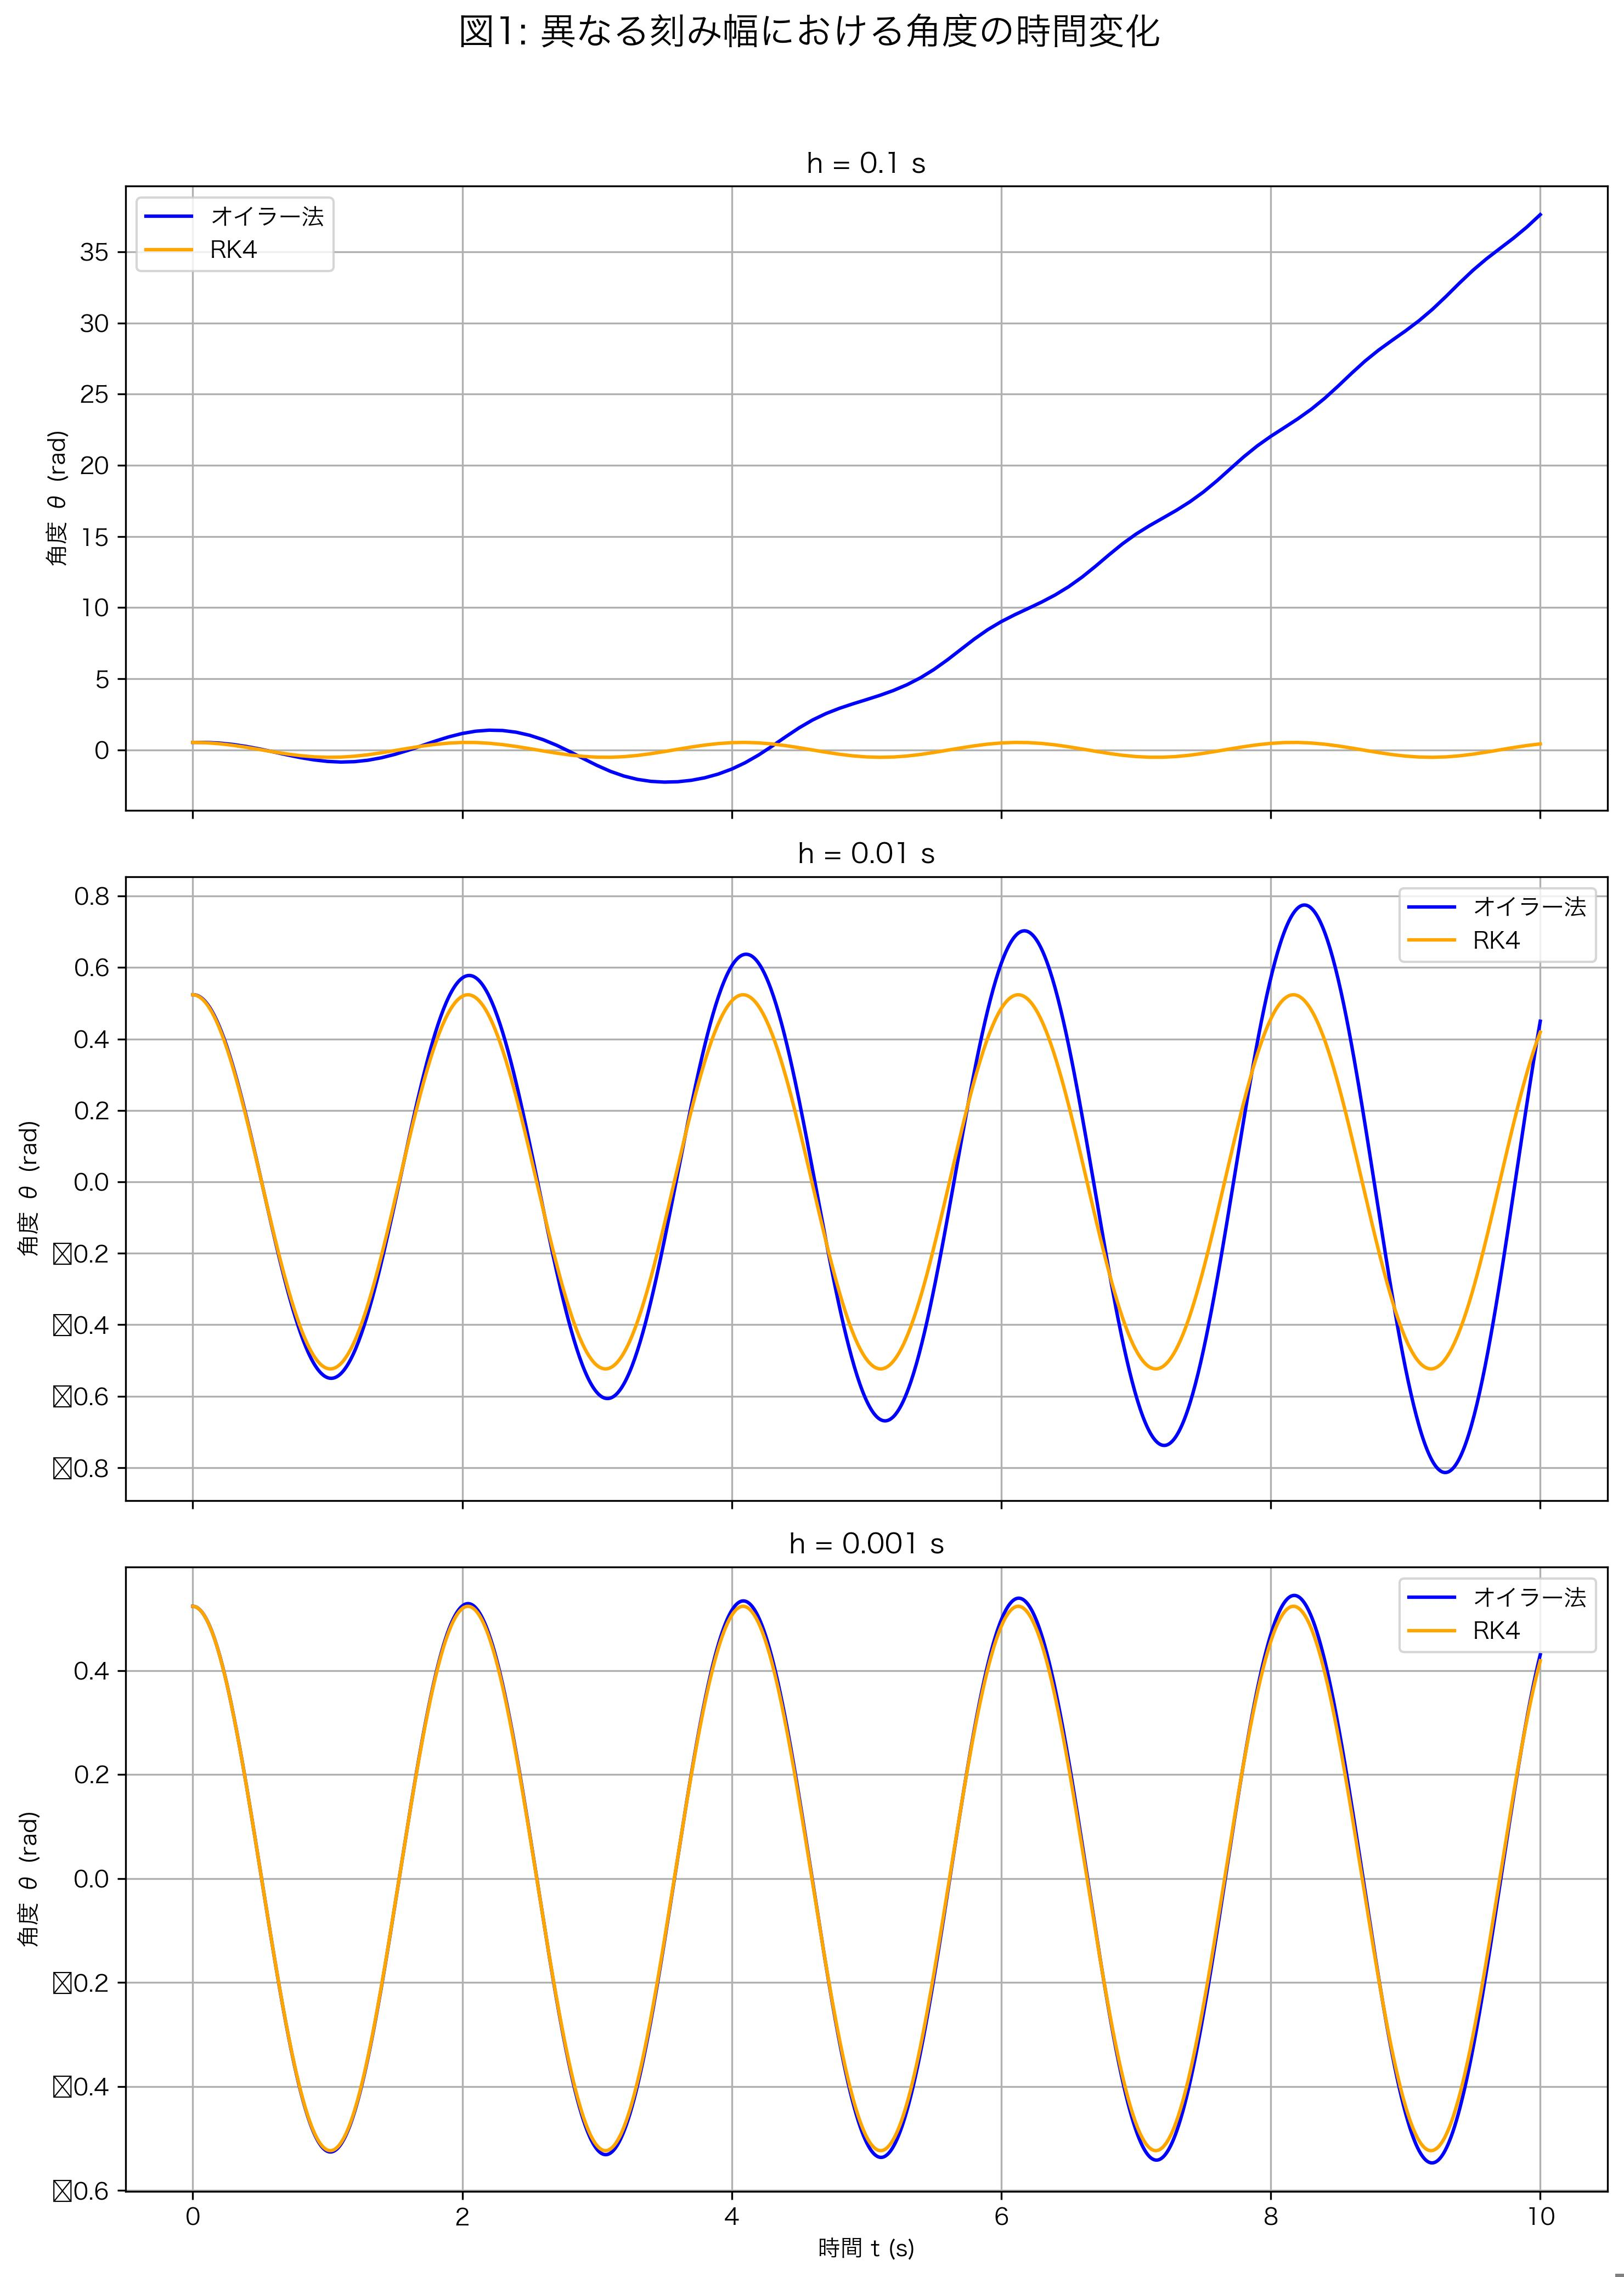
\includegraphics[width=\textwidth]{図1_角度の時間変化.jpg}
  \caption{3つの異なる刻み幅(上から $h=0.1$, $h=0.01$, $h=0.001$)における、オイラー法とRK4による角度 $\theta$ の時間変化。横軸は時間 $t$ (s)、縦軸は角度 $\theta$ (rad) を示す。}
  \label{fig:angle}
\end{figure}

\begin{figure}[htbp]
  \centering
  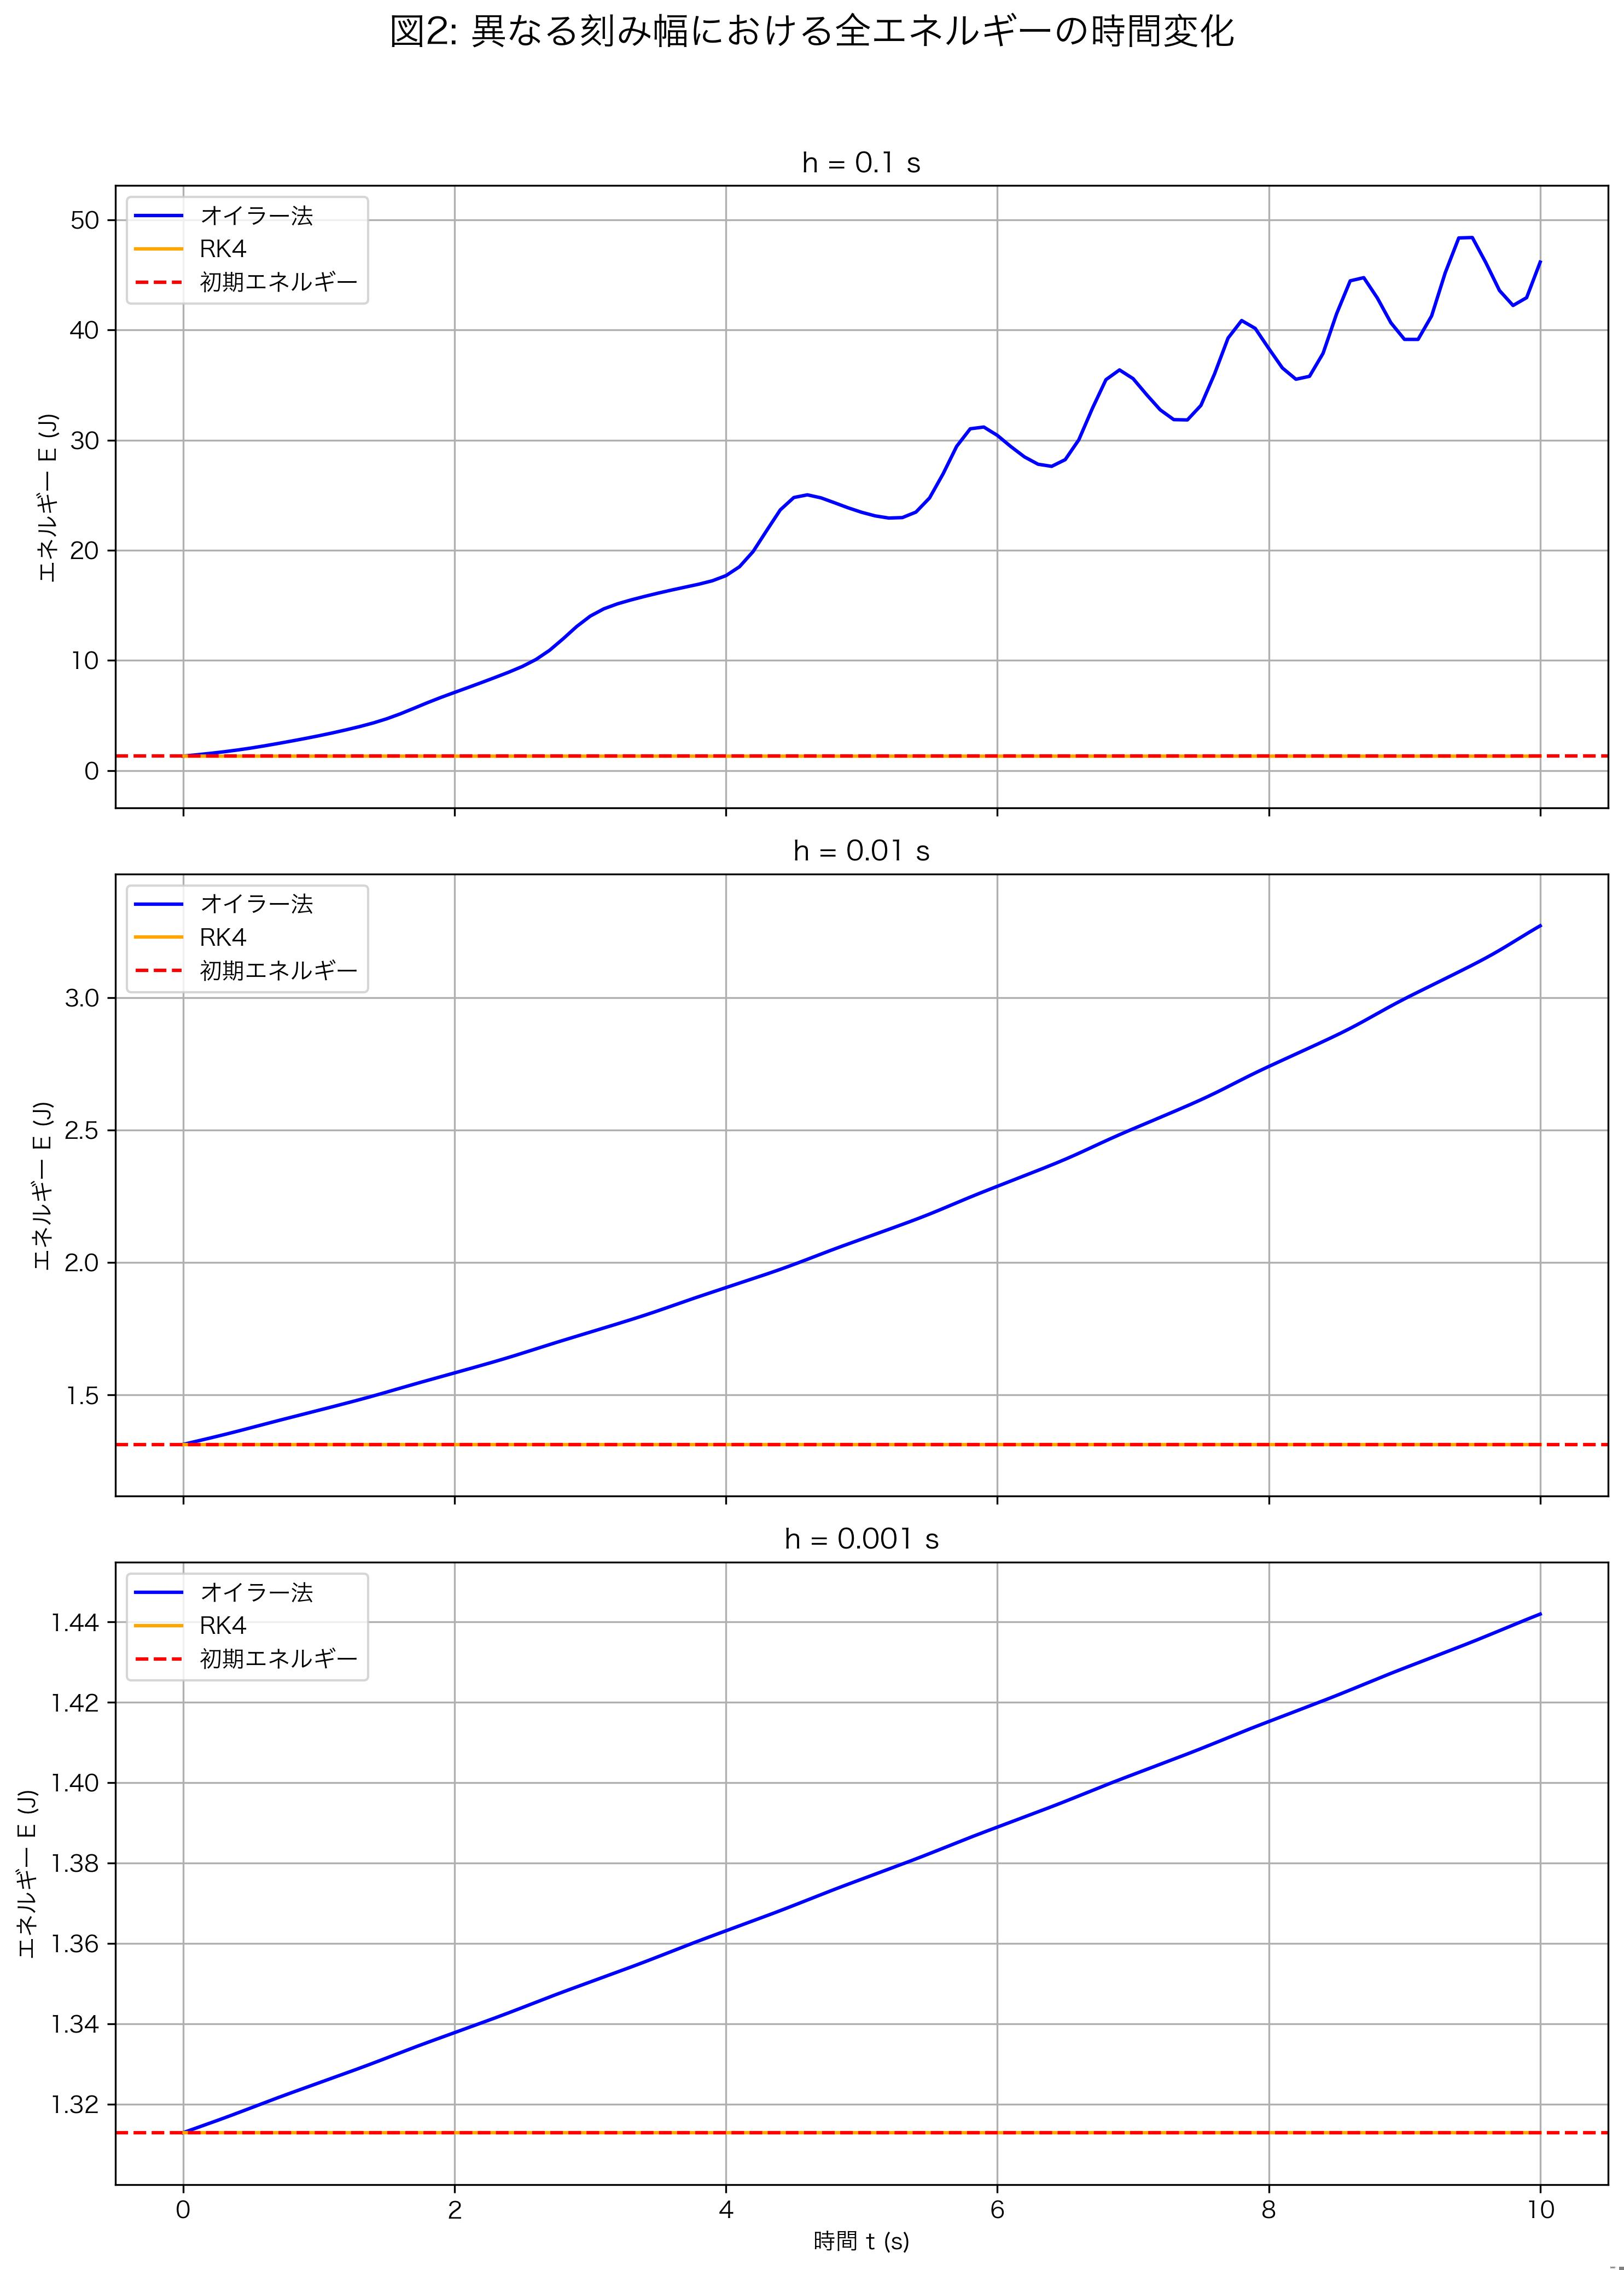
\includegraphics[width=\textwidth]{図2_エネルギーの時間変化.jpg}
  \caption{3つの異なる刻み幅(上から $h=0.1$, $h=0.01$, $h=0.001$)における、オイラー法とRK4で計算された全力学的エネルギー $E$ の時間変化。横軸は時間 $t$ (s)、縦軸はエネルギー $E$ (J) を示す。破線は初期エネルギーの値を示す。}
  \label{fig:energy}
\end{figure}

\clearpage

\section{考察}

\subsection{解の精度と安定性の比較}
図\ref{fig:angle}は、両手法の解の精度と安定性の違いを明確に示している。$h=0.1$ の場合、オイラー法による解は振幅が際限なく増大し、物理的にありえない挙動を示す。これは、オイラー法が容易に破綻することを示している。一方、RK4は安定した周期的振動を維持している。刻み幅を $h=0.01$ に狭めると、オイラー法の解は改善されるが、RK4の解と比較すると位相が徐々にずれていく。$h=0.001$ にすると、オイラー法の解はRK4の解に視覚的に近くなるが、表\ref{tab:results}の最終角度を見ると依然として誤差の蓄積が見られる。対照的に、RK4は $h=0.1$ ですら安定した解を生成し、$h=0.01$ と $h=0.001$ の結果はほぼ完全に一致しており、非常に速く真の解に収束することを示している。

\subsection{物理法則の再現性:エネルギー保存}
図\ref{fig:energy}は、シミュレーションの物理的な妥当性を評価するための決定的な証拠を提供する。オイラー法では、すべての刻み幅において、計算された全力学的エネルギーが時間とともに単調に増加している。$h=0.1$ の場合、10秒後には初期エネルギーの約35倍にまで増加しており、シミュレーションが物理的現実から完全に乖離していることを示している。これは、オイラー法が系の軌道を常に外側へ更新してしまうアルゴリズムの構造的欠陥に起因する。対照的に、RK4ではエネルギーは初期値の周りで非常に小さく振動するのみで、系統的な増加や減少は見られない。特に $h=0.01$ と $h=0.001$ では、エネルギーは極めて高い精度で保存されており、RK4が系の物理法則を忠実に再現する能力を持つことがわかる。

\subsection{数値誤差の理論的考察}
実験で観測された性能差は、両手法の理論的な精度の次数の違いによって説明できる。オイラー法の大域離散化誤差は $O(h)$、RK4のそれは $O(h^4)$ である。これは、刻み幅 $h$ を1/10にすると、オイラー法の誤差は約1/10に減少するのに対し、RK4の誤差は約1/10000に減少することを意味する。この圧倒的な収束率の違いが、RK4がはるかに少ない計算ステップで高精度な解を得られる理由である。この精度の違いは、ステップ内で複数回傾きを評価し加重平均するRK4の洗練されたアルゴリズム構造に起因する。

\subsection{計算効率と精度のトレードオフ}
1ステップあたりの計算量はRK4がオイラー法の4倍であるが、「目標とする精度を達成するための総コスト」で比較すると、多くの場合RK4が優れる。本実験が示すように、実用的な精度を求める場合、RK4はより大きな刻み幅を使えるため、総計算量においてオイラー法よりも効率的になる。低精度でよい一部のケースを除き、RK4の方が計算効率と精度のバランスに優れた手法であると言える。

\section{結論}
本研究では、オイラー法と4次ルンゲ・クッタ法(RK4)を実装し、単振り子の運動シミュレーションを通じて両者の性能を比較・評価した。
\begin{enumerate}
    \item \textbf{オイラー法}は、実装が容易だが精度が低く、特に力学的エネルギーを保存できないという致命的な欠陥を持つ。そのため、保存則が重要な物理系の長期シミュレーションには不適切である。
    \item \textbf{4次ルンゲ・クッタ法(RK4)}は、アルゴリズムは複雑だが4次という高い精度を持ち、粗い刻み幅でも安定かつ高精度な解を生成する。特に、力学的エネルギーを極めて高い精度で保存する能力があり、物理法則に忠実なシミュレーションが可能である。
    \item 計算効率の観点からは、目標とする精度を達成するために必要な総計算量では、多くの場合RK4がオイラー法を上回る。
\end{enumerate}
総じて、非線形な物理系を正確にシミュレーションするためには、問題の特性に適した高次精度で安定した数値解法を選択することが極めて重要である。オイラー法は教育的な導入としては有用だが、実際の科学技術計算においては、RK4のようなより洗練された手法を用いることが、信頼性の高い結果を得るための必須要件であると言えよう。

\begin{thebibliography}{9}
    \bibitem{mitsui} 三井 斌友 (2003). 『常微分方程式の数値解法』. 岩波書店.
    \bibitem{yamamoto} 山本 哲朗 (2003). 『数値解析入門 [増訂版]』. サイエンス社.
\end{thebibliography}

\appendix
\section{プログラムコード}
\begin{lstlisting}[caption={Python code used for numerical experiments, tables, and graphs in this study}, label={lst:code}]
import numpy as np
import matplotlib.pyplot as plt
import matplotlib as mpl

# 日本語フォントの設定
plt.rcParams['font.family'] = 'sans-serif'
plt.rcParams['font.sans-serif'] = ['Hiragino Sans GB', 'Arial', 'Helvetica', 'Yu Gothic', 'Meiryo', 'MS Gothic']


# 数式フォントの設定
mpl.rcParams['mathtext.default'] = 'regular'

# --- グローバル設定 ---
# 物理定数
G = 9.8  # 重力加速度 (m/s^2)
L = 1.0  # 振り子の長さ (m)
M = 1.0  # 質点の質量 (kg)


# 初期条件
THETA_0 = np.pi / 6  # 初期角度 30度 (rad)
OMEGA_0 = 0.0        # 初期角速度 (rad/s)

# シミュレーション時間
T_START = 0.0
T_END = 10.0

# --- 連立1階常微分方程式の定義 ---
# y = [theta, omega]
# dy/dt = f(t, y)
def f(t, y):
    """
    単振り子の運動方程式を記述するベクトル関数。
    Args:
        t (float): 時刻 (未使用だが、一般的なソルバーのインターフェースに合わせる)
        y (np.ndarray): 状態ベクトル [theta, omega]
    Returns:
        np.ndarray: 状態ベクトルの時間微分 [d(theta)/dt, d(omega)/dt]
    """
    theta, omega = y
    return np.array([omega, -(G / L) * np.sin(theta)])

# --- エネルギー計算関数 ---
def calculate_energy(y):
    """
    与えられた状態ベクトルから全力学的エネルギーを計算する。
    Args:
        y (np.ndarray): 状態ベクトル [theta, omega]
    Returns:
        float: 全力学的エネルギー (J)
    """
    theta, omega = y
    kinetic_energy = 0.5 * M * (L * omega)**2
    potential_energy = M * G * L * (1 - np.cos(theta))
    return kinetic_energy + potential_energy

# --- 数値解法ソルバー ---
def euler_step(f_func, t, y, h):
    """オイラー法による1ステップ計算"""
    return y + h * f_func(t, y)

def rk4_step(f_func, t, y, h):
    """4次ルンゲ・クッタ法による1ステップ計算"""
    k1 = h * f_func(t, y)
    k2 = h * f_func(t + h / 2, y + k1 / 2)
    k3 = h * f_func(t + h / 2, y + k2 / 2)
    k4 = h * f_func(t + h, y + k3)
    return y + (k1 + 2 * k2 + 2 * k3 + k4) / 6

# --- シミュレーション実行関数 ---
def run_simulation(h, solver_func):
    """
    指定された刻み幅とソルバーでシミュレーションを実行する。
    Args:
        h (float): 時間刻み幅
        solver_func (function): 使用するソルバー関数 (euler_step or rk4_step)
    Returns:
        tuple: (時間配列, 角度配列, エネルギー配列)
    """
    time_points = np.arange(T_START, T_END + h, h)
    num_steps = len(time_points)
    
    y_history = np.zeros((num_steps, 2))
    y_history[0] = np.array([THETA_0, OMEGA_0])  # 初期条件を設定
    
    energy_history = np.zeros(num_steps)
    energy_history[0] = calculate_energy(y_history[0])
    
    for i in range(num_steps - 1):
        y_history[i+1] = solver_func(f, time_points[i], y_history[i], h)
        energy_history[i+1] = calculate_energy(y_history[i+1])
        
    theta_history = y_history[:, 0]
    return time_points, theta_history, energy_history

# --- メイン処理 ---
if __name__ == '__main__':
    H_LIST = [0.1, 0.01, 0.001]
    
    # --- 表1のデータ生成 ---
    initial_energy = calculate_energy(np.array([THETA_0, OMEGA_0]))
    print("表1: 各手法と刻み幅における最終時点(t=10s)の角度とエネルギー")
    print(f"(初期エネルギー E_0 = {initial_energy:.6f} J)")
    print("| 手法 (Method) | 刻み幅 h (s) | 最終角度 θ(10) (rad) | 最終エネルギー E(10) (J) |")
    print("|:---|:---|:---|:---|")
    
    solvers = {'オイラー法': euler_step, 'RK4': rk4_step}
    results_for_table = {}

    for name, solver in solvers.items():
        for h in H_LIST:
            t, theta, energy = run_simulation(h, solver)
            print(f"| {name} | {h:<12} | {theta[-1]:.6f} | {energy[-1]:.6f} |")
            results_for_table[(name, h)] = (t, theta, energy)

    # --- 図1と図2のプロット生成 ---
    fig_angle, axes_angle = plt.subplots(3, 1, figsize=(10, 15), sharex=True)
    fig_energy, axes_energy = plt.subplots(3, 1, figsize=(10, 15), sharex=True)
    
    fig_angle.suptitle('図1: 異なる刻み幅における角度の時間変化', fontsize=16, y=0.92)
    fig_energy.suptitle('図2: 異なる刻み幅における全エネルギーの時間変化', fontsize=16, y=0.92)

    for i, h in enumerate(H_LIST):
        # オイラー法の結果を取得
        t_e, theta_e, energy_e = results_for_table[('オイラー法', h)]
        # RK4の結果を取得
        t_r, theta_r, energy_r = results_for_table[('RK4', h)]
        
        # 図1: 角度のプロット
        axes_angle[i].plot(t_e, theta_e, label='オイラー法', color='blue')
        axes_angle[i].plot(t_r, theta_r, label='RK4', color='orange')
        axes_angle[i].set_title(f'h = {h} s')
        axes_angle[i].set_ylabel('角度 $\\theta$ (rad)')
        axes_angle[i].grid(True)
        axes_angle[i].legend()
        
        # 図2: エネルギーのプロット
        axes_energy[i].plot(t_e, energy_e, label='オイラー法', color='blue')
        axes_energy[i].plot(t_r, energy_r, label='RK4', color='orange')
        axes_energy[i].axhline(y=initial_energy, color='red', linestyle='--', label='初期エネルギー')
        axes_energy[i].set_title(f'h = {h} s')
        axes_energy[i].set_ylabel('エネルギー E (J)')
        axes_energy[i].grid(True)
        axes_energy[i].legend()
        # Y軸の範囲を調整して変動を見やすくする
        energy_max = max(np.max(energy_e), np.max(energy_r))
        energy_min = min(np.min(energy_e), np.min(energy_r))
        padding = (energy_max - energy_min) * 0.1
        axes_energy[i].set_ylim(min(initial_energy, energy_min) - padding, energy_max + padding)

    axes_angle[-1].set_xlabel('時間 t (s)')
    axes_energy[-1].set_xlabel('時間 t (s)')
    
    fig_angle.tight_layout(rect=[0, 0, 1, 0.9])
    fig_energy.tight_layout(rect=[0, 0, 1, 0.9])

    fig_angle.savefig('図1_角度の時間変化.jpg', dpi=300, bbox_inches='tight')
    fig_energy.savefig('図2_エネルギーの時間変化.jpg', dpi=300, bbox_inches='tight')


    plt.show()


</lstlisting>

\end{document}